\chapter{Project Analysis}
\label{chap:prjan}

\section{Project roadmap}
\label{chap:prjan:sec:prjsche}

Prior to starting with the actual implementation of the technical SFC
specification, we carried out a feasibility analysis in order to estimate the
required time and activities involved. A pragmatic estimated concluded that a
six months period was needed in order to create a working proof of concept
(PoC) that would allow us to perform tests and, in general, to have feedback
about the solution.

\subsection{Scheduled timeline}
Since our knowledge about the technologies was very poor at the beginning, we
preferred to invest a good chunk of time on studying them, in order to
understand the literature material and industry PoCs and to choose accordingly
what we really needed. Additionally, at the end of this phase we thought it was
necessary to try these products to see if they really fitted our necessities.
After this phase, we planned to actually start implementing the missing
components so to create and fulfill the requirements defined in Section~
\ref{chap:prjan:sec:req}. Since we had prior knowledge on the Java C/C++
languages, we estimated an eight-week period for coding and software
implementation. After that, two weeks were calculated in order to perform tests
and gather metrics about the system built and to see how much the job already
done satisfied our expectations. Finally, we estimated four weeks to put and
write down all the information and considerations we gathered during the thesis.

\subsection{Actual timeline}
Unfortunately, many difficulties slowed our project development down since the
very beginning. The total time we estimated to carry out all the planned
requirements was of $37$ weeks, namely nine months circa. Many problems emerged
during the study of the technologies that revealed to be more complicated than
expected, especially since some frameworks were more intricate to deploy and to
try them out. Time was wasted to obtain resources from the University that were
not initially planned for. On top of that, we encountered little bugs we had to
manually fix, like in the Floodlight
Controller\footnote{See \url{https://github.com/floodlight/floodlight-webui/pull/10}},
that additionally slowed our technologies exploration. This unplanned digging
in other projects' code cost us time and resources, delaying the first phase of
eight
weeks, for a total of $17$ weeks. The software implementation revealed to be
irksome too. We ended up underestimating the time required for this phase,
because
we did not consider all the issues related to work with system calls. Moreover,
we had to implement more components than planned, in order to be able to
actually transmit data between two senders. In a nutshell, the additional time
required was of eight weeks, for a total of $16$ weeks. In the end, the time to
write
down the thesis was limited, and we had to write it down in a
total of two weeks, instead of the four initially planned.

\section{Requirements}\label{chap:prjan:sec:req}
In the following section are described the main requirements of this project.

\begin{longtable}[c]{p{0.32\textwidth}p{0.68\textwidth}}
\hline
\multicolumn{1}{c}{\textbf{Requirement}}                               &
\multicolumn{1}{c}{\textbf{Description}}                               \\ \hline
\endhead
%
\hline
\endfoot
%
\endlastfoot
%
1. Automatic NFVI creation and configuration &
It must be possible to create the environment on which the SFC will be deployed
in an automatic manner. The system must support Docker container and must be
deployed on a clustered environment. \\
2. Implementation of chain orchestration and management tools &
The final work must be comprehensive of a minimal software implementation that
allows the deployment, the management and the orchestration of VNFs and their
lifecycle. \\
3. Automatic configuration of chain orchestration and management tools &
Software instrumentation for VNFs and SFCs management must be configured
automatically, at startup. \\
4. Developing software for manual SFC deployment &
An instrumentation to deploy a chain of containers in which VNFs can run must
be developed. These containers must be able to communicate with each
other. \\
5. VNF fault management &
The system must be able to automatically recover a faulty container. \\
6. VNF scalability &
The system must be able to scale the number of containers implementing a
function, both augmenting and decrementing their replicas. \\
7. SFC definition saving &
The system must be able to save a definition of a chain \\
8. Chain definition deploy/stop/update & The system must be able to allow the
deployment of a chain from a saved definition, stop a running SFC and update
it. \\
\hline
\caption{Table of requirements}
\label{chap:prjan:tab:req}\\
\end{longtable}

\section{Technology evaluation}

\subsection{Openstack platform for cloud computing}
\begin{figure}[t]
  \centering \includegraphics[scale=0.58]{openstack_logo}
  \caption{Openstack logo}
  \label{chap:prjan:img:openstack_logo}
\end{figure}
Openstack was released in 2010 and developed by Rackspace Hosting and
NASA~\cite{openstackWebsite}. It is a free and open-source platform for cloud
computing released under Apache license. It is mostly developed to be an IaaS,
installing the software on bare-metal resource to virtualize physical resource
that can be eventually made available to end-users. It has a modular
architecture composed be different components, most significant for the project:
\begin{itemize}
\item \emph{Nova} manages the computing resources;
\item \emph{Glance} manages server images;
\item \emph{Keystone} is accountable of the identities;
\item \emph{Horizon} dashboard to manage Openstack;
\item \emph{Neutron} manages networking;
\item \emph{Cinder} provides persistent storage to compute instances.
\end{itemize}
then other components can be added.

Openstack usage in this project is twofold. All machines on which we deployed
and tested our solution where virtual machine running on top of the University
Openstack instance. Moreover, in the early stages of the project, we performed
a Devstack (Openstack version that requires less resources, released for
developers that have to work with Openstack, it is not suitable for a production
environment) installation on VM running on the Openstack instance of
the University. Since in this installation we had full access to all the
functionalities of the software (at the contrary that in the other instance), we
were able to install all the components that we wanted and to evaluate different
technologies.


\subsection{Kubernetes containers orchestrator}
\begin{figure}[h]
  \centering \includegraphics[scale=0.35]{kubernetes_logo}
  \caption{Kubernetes Logo}
  \label{chap:intro:img:k8s_logo}
\end{figure}
Kubernetes was released in 2014 and developed by Google. It is an open-source
orchestrator for containers that allows automating deployment, scaling and
management, written in Go. This product is thought to provide the simplicity of
management of a Platform as a Service (PaaS), mixed with flexibility of the
IaaS, allowing the portability on different infrastructure provides. Differently
of usual PaaS it does not operates at hardware level, but at container level,
creating a virtualized layer without explicitly concerning with physical
resources. In a Kubernetes cluster, real hosts are called Nodes, and they can be
assigned with different roles or specifications. One or more Nodes must have the
role of \emph{master}. Master has the task to orchestrate containers deployed. 

Even if Kubernetes is container-centric it allow to change the virtualization
software and use for instance virtual machine software.

It was the most important technology that we used in the project, and one of the
most time consuming in terms of study, installation and configuration. Most of
the components of our proposal run on Kubernetes and the other were developed to
interact with it. How we utilize Kubernetes is explained in
Section~\ref{chap:archimpl} and in Section~\ref{chap:impl}. Instead in
Appendix~\ref{kubernetes} there is a guide on Kubernetes main concepts and how
to install it, that we create during the project.

\subsection{Docker operating-system-level virtualization}
\begin{figure}[t]
  \centering \includegraphics[scale=0.7]{docker_logo}
  \caption{Official Docker logo}
  \label{chap:intro:img:docker_logo}
\end{figure}
Docker was released in 2013 and developed by Docker Inc. It is an open source
software that operates the operating-system-virtualization (OS-virtualization,
also called \emph{containerization}), written in Go. This typology of
virtualization exploit the kernel level feature of allowing the existence of
multiple isolated user-space instances: in this way all containers running on
the same host utilize the same operating system kernel. That is why containers
are more lightweight compared to virtual machines, in which even the kernel is
duplicated, requiring more resources. Docker is based on a previous OS-level
virtualization technology that is the Linux Containers (LXC). LXCs utilize the 
\texttt{cgroups} functionality that allows limitation and prioritization of
resources (CPU, memory, block I/O, network, etc.) and namespace isolation
functionality that allows complete isolation of an applications. Docker extends
LXC with a kernel and an application-level API that together run processes in
isolation. Docker containers are created using base images, that can define just
the OS fundamentals, or it can consist of a prebuilt application stack.
Commands can be executed manually or automatically using Dockerfiles.

\emph{Docker Engine} is a client-server application mainly composed by i) a
server \texttt{dockerd}, that is a daemon process, ii) a REST API that specifies
interfaces that programs can use to talk to the daemon and iii) a command line
interface client (that is the \texttt{docker} command).

\emph{Docker Hub} instead is the Software as a Service (SaaS) platform that
allows to share and manage images created.

In the thesis this technology was used to create images in which run our
components that will be deployed on Kubernetes. Images where automatically build
taking advantage of Docker Hub from the Dockerfiles specified in our Github
repository. This also ease the deployment on Kubernetes of components, since
images where retrieved from the Docker SaaS service.

\subsection{Docker Compose tool for multi-container applications}
\begin{figure}[t]
  \centering 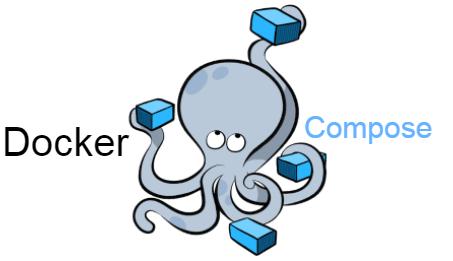
\includegraphics[scale=0.5]{dockercompose_logo}
  \caption{Docker Compose logo}
  \label{chap:intro:img:docker_logo}
\end{figure}
Docker Compose was released in 2013 and developed by Docker Inc. It is a tool
to define and run multiple-container applications, automating their launch.
Application configuration is specified using a single YAML file, that make
easier to specify interaction among the containers of which it is composed.
Pieces in which the application can be decomposed are called
\emph{services}. They does not specify only the image that has to be run but
it defines even the configuration (such as ports to use or resource limitation).
Docker Compose also enable the capability to scale the number of running
instances of the same container. This product has other features. It creates
different environments for each Compose definition and preserves data used by 
certain service. Thus, if at startup it finds any containers from previous runs,
it copies the volumes from the old to the new one, avoiding data loss. Finally,
it caches the configuration used to create a container and if during
the restarting phase of a service there are no changes, Compose re-uses the
existing ones.

In the project this tools was used to develop and test components in a
controlled environment. Also, before deploying new parts of the system on
Kubernetes, their integration with the other components were test on Compose,
even because deploying a new component on Kubernetes is quite a cumbersome task,
requiring both the YAML definition of the application and that images are
available (or updated) on Docker Hub.

\subsection{Docker Swarm clustering system}
\begin{figure}[t]
  \centering 
\includegraphics[scale=1.2]{dockerswarm_logo}
  \caption{Docker Swarm logo}
  \label{chap:intro:img:docker_logo}
\end{figure}
Docker Swarm was released in 2014 and developed by Docker Inc. It allows to
manage multiple Docker Engines clustered and seen as a single logical unit.
Physical hosts, named Nodes, are splitted into \emph{managers}, that have the
task to manage the cluster, maintaining cluster state and orchestrating services
and Swarm API calls, and \emph{workers}, that run containers. Docker CLI can
be used to orchestrate containers within a swarm, making its use transparent as
it makes transparent the underlying infrastructure. It offers scalability
features and make possible the definition of an overlay network for services.
Application can be deployed on a Swarm describing them using Docker Compose,
moving this tool from a one node environment to a clustered one.

This technology was evaluated choosing the clustered environment to which deploy
out solution. Finally, the choice was Kubernetes because it has more
customization capabilities, that make it more flexible. Moreover, Kubernetes has
auto-scaling features that are not directly available in Docker Swarm. This is
can be really important in case of deploying SFC in environments in which
traffic load can change dramatically. Moreover, Kubernetes supports up to $5000$
nodes, instead only Swarm up to $1000$. Finally, more information and
documentation on Kubernetes was found.

\subsection{OpenvSwitch multilayer virtual switch}
\begin{figure}[h]
 \centering 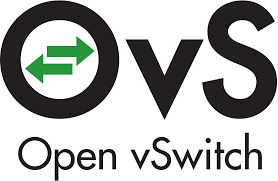
\includegraphics[scale=0.45]{ovs}
 \caption{OpenvSwitch logo}
 \label{chap:prjan:img:ovs_logo}
\end{figure}
OpenvSwitch (OVS) was developed in 2009, is an open-source implementation,
released under Apache 2.0 license, of a multi-layer virtual switch. It provides
a switching stack for hardware virtualization. It was designed to enable network
automation using programmatic extension and support a variety of different
network protocols. It support the possibility of bridging traffic between a
virtualized environment, both using virtual machines and container, and the
outside world. It supports OpenFlow protocol and it can be used in conjunction
of a \emph{controller} in SDN context to define traffic routing. In the latter
scenario it also allows to tie together all the virtual machines instances
of a server and it serves as entrypoint to overlay networks running on top of
physical networks. It is also used in redirect traffic in service chaining use
cases.

\subsection{Floodlight open SDN controller}
\begin{figure}[h]
 \centering 
\includegraphics[scale=0.6]{floodlight}
 \caption{Floodlight logo}
 \label{chap:prjan:img:floodlight_logo}
\end{figure}
Floodlight was released in 2011 and it is an open-source, community-developed
project, distributed under Apache 2.0 license. It is an OpenFlow Java-based
Controller that works both with physical and virtual switches that support the
OpenFlow protocol. Its goal is the traffic flows orchestration in
SDN: Floodlight provides the possibility to define rules to route traffic, that
it will manage, applying the necessary instructions to the infrastructure on how
traffic has to be handled.

This product, in combination with OpenvSwitch was studied in the first part of
the thesis, to better understand how some other SFC proposals and SDN solutions
work and route traffic. It was lately abandoned due to architectural and
implementation choices, that moved the task of routing traffic to other
components.

\subsection{Openbaton NFV MANO-compliant framework}
\begin{figure}[h]
  \centering \includegraphics[scale=0.45]{openbaton_logo}
  \caption{Openbaton logo}
  \label{chap:prjan:img:openbaton_logo}
\end{figure}
Openbaton is developed by the Institute Fraunhofer and it is an open-source
platform that supply an implementation of the ETSI NFV MANO specification. It
can be either installed as a normal program or run into containers from a Docker
Compose definition. This framework is capable to orchestrate network services on
different NFV Infrastructures. It can manage different VNFs ecosystems thanks
its Generic VNFM and it is capable to compose them. It leaves to developers the
possibility to integrate new VNFM using plugins and the APIs and SDKs
they developed that support different languages. It also supports the VNF
deployment on different VIMs, like Amazon Web Services and Openstack, allowing
even in that case the possibility to increase the number of supported VIMs
creating new drivers. Places to which VNF can be deployed are registered as
Point of Presence (POP), providing necessary access information. Openbaton
supports VNFs auto-scaling management, based on monitoring information and fault
management for failures that can occur on different levels. Monitoring
is implemented with a plugin that exploit Zabbix\footnote{Software to monitor
performance of an IT infrastructure \url{https://www.zabbix.com/}}. Lifecycle of
VNFs compatible with this platform can be completely handled even from the
dashboard. It also has a Marketplace to which Openbaton-compatible VNFs can be
downloaded. Custom VNFs can be stored and run on demand following the Topology
and Orchestration Specification for Cloud Applications (TOSCA) definition or
YAML files.

Openbaton was taken into account as ETSI compliant MANO for our solution, both
because of its flexibility and possibility to extend it with plugins. Moreover
it could allow us to register new VIM typologies. Lately due to the difficulties
to create a Kubernetes driver was abandoned.

\subsection{Dnsmasq network infrastructure tool}
\begin{figure}[h]
  \centering 
\includegraphics[scale=0.6]{dnsmasq_logo}
  \caption{Dnsmasq logo}
  \label{chap:prjan:img:dnsmasq_logo}
\end{figure}
Dnsmasq is an open source project, started in 2001~\cite{dnsmasqweb}. Its
features includes the possibility to serve as DNS, DHCP or router advertisement
and network boot. Dnsmasq is designed to have a small footprint memory, and it
is suited for medium to small network infrastructures. Along with the DNS
server, it has the possibility to perform request caching, to speed up
additional requests of the same type. On top of that, it provides different
compilation options in order to eliminate unused features at compile time.

\subsection{Tacker: Openstack VNF Manager and NFV Orchestrator}
Tacker is an open-source software for NFV Orchestration, released under Apache
2.0 license, based on ETSI MANO Architectural Framework. This product is
implemented to both work as Generic VNF Manager and NFV Orchestrator, enabling
deployment and management of VNFs on infrastructures like Openstack. It can be
added to an existing Openstack installation as a additional component. As
Openbaton handle the entire lifecycle of VNF and monitor their status using
Zabbix. Another analogy with Openbaton is that VNFs can be recorded following
the TOSCA definition. Differently to Openbaton, instead, it seem to be designed
to support different typologies of VIMs (as Kubernetes for example). 
